\documentclass[a4paper,11pt]{article}
\usepackage[T1]{fontenc}
\usepackage{fullpage,graphicx,psfrag,amsmath,amsfonts}
\usepackage[utf8]{inputenc}
\usepackage[english]{babel}
\usepackage{lipsum}
\usepackage{url}
\usepackage{amsmath}
\usepackage{bm}
\usepackage{listings}
\usepackage{float}
\usepackage{fancyvrb}
\usepackage{enumitem}
\usepackage{kpfonts}
\usepackage{tikz}
\usetikzlibrary{shapes,arrows}
\usepackage{mathpazo}
\begin{document}
\author{Filippo Grotto VR460638}

\title{Bechmarking control algorithms with current saturation aware references \\[1ex] \large Robot Programming and Control}

\maketitle
\tableofcontents

\section{Introduction}
The aim of Forecast project \cite{Forecast} is to provide a testbed to benchmark control algorithms and get in this way comparable results especially in the context of force control algorithms. The procedure uses several performances indicators to assess the controller in use such as static error, dynamic error, overshoot and bandwidth. The latter is estimated using a sinusoidal function that increments frequency over time (e.g. 1 to 10Hz in 10 seconds) until we reach -3db over the desired reference. However this estimation suffers from the presence of saturation of the motor used to drive the experiments making the result about the controller not as general as we want. In the following section we will propose a method to reduce the amplitude of the reference signal before reaching the motor saturation in order to get a much more precise bandwidth estimation using general transfer function methods in case of fully linear systems.

\newpage
\section{Noise Sensitivity Function}
If we consider the general feedback system in Fig.\ref{fig:feedback}. There are lots of transfer function that we are possibile to define depending on our input-outputs pairs. In our cases we will consider $F(s)=1$. 

\begin{figure}[H]
\begin{center}
\includegraphics[width=0.6\textwidth]{images/feedback.png}
\end{center}
\caption{A general SISO feedback system taken from \cite{scientist}}
\label{fig:feedback}
\end{figure}

\noindent We are actually interested in having the relation between the input of the system $r$ and the control input $u$ in order to know when the current saturation is reached. We will assume our $P(s)$ plant known since we can identify all the parameters of our DC motors assuming it to be a linear system.
\begin{equation}
  CS(s) = \frac{C(s)}{1+C(s)P(s)}
\end{equation}

\noindent The procedure proposed for the current saturations is derived considering the motor saturation $u_{sat}$ usually provided in the datasheets:
\begin{equation}
  \frac{u}{u_{sat}} < 1
  \label{eqn:current_sat}
\end{equation}

\noindent The equation \eqref{eqn:current_sat} holds since we want $u$ to not overcome the provided saturation. However a more strict condition can be imposed. We can then write:

\begin{equation}
  \frac{u}{u_{sat}} = |CS(s)| \frac{r}{u_{sat}}
\end{equation}

\noindent Considering the worst case scenario when $u/u_{sat}=1$ we can derive:

\begin{equation}
  r < \frac{u_{sat}}{|CS(s)|}
  \label{eqn:saturation_limit}
\end{equation}

\noindent An equivalent condition for unitary input is:
\begin{equation}
  \frac{|CS(s)|}{u_{sat}} < 1 (0db)
  \label{eqn:saturation_limit2}
\end{equation}

\noindent Note that equation \eqref{eqn:saturation_limit} and \eqref{eqn:saturation_limit2} use mixed time and laplace domain notations. In the following sections only the magnitude of the transfer function will be considered. 

\newpage
\section{Control Architectures}

Our aim is to replace the input of the different architectures with a correctly scaled sinusoidal function (sweep) which guarantees that motor saturation is not exceeded during the simulated experiment. To do so the signal is firstly processed by some matlab code which scaled it using the presented equations secondly the simulink model is considered using the generated signal and current/tau is considered. 
\bigskip

\noindent The following code was used to generate the reference signal:

\bigskip
\begin{lstlisting}
  % Calculate time and frequencies vectors (they must have the same length)
  t = start_T:dt:end_T;
  freq = start_freq + ((end_freq-start_freq)/duration * t);
  
  % Build original swept function
  sweep = amplitude * chirp(t, start_freq, end_T, end_freq, 'linear', -90);
  
  % Compute the magnitude vector /m
  [magnitude_vector,~] = bode((CS*amplitude)/(u_sat), 2*pi*freq);
  
  % Calculate deamplification factor only when the magnitude is larger than
  % 0db (1 in linear scale).
  deamplification = zeros(1,size(magnitude_vector, 3));
  for i = 1:size(magnitude_vector,3)
      if magnitude_vector(:,:,i) >= 1 
          deamplification(i) = amplitude/magnitude_vector(:,:,i);
      else
          deamplification(i) = amplitude;
      end
  end
  
  % Build the suggested sweep
  suggested_sweep = deamplification .* chirp(t, start_freq,
                                      end_T, end_freq, 'linear', -90);
\end{lstlisting}

\smallskip
\noindent Briefly, the idea is to use the magnitude of the trasfer function \eqref{eqn:saturation_limit3} to scale the reference only when we exceed 0db (1 in linear scale). That means we allow the user to define the reference and we scale only when we can't guarantee the saturation limits (forcing, in that scenario, the maximum current available).

\smallskip
\begin{equation}
  \frac{|CS(s)|amplitude}{u_{sat}} 
  \label{eqn:saturation_limit3}
\end{equation}

\newpage

\subsection{Parameters Used}

\bigskip
The parameters used for the motor comes from direct identification of a maxon DCX22L, in particular $J_m = 0.0064Kgm^2$, $d_m = 0.0068Nms$, $K_t = 1.46$ and $u_{sat} = 2.26A$. The controller used for all the architectures is a PID/PD controller with different parameters.

\bigskip
\subsection{Position Control}
Let's consider a basic position control architecture for a linear motor model considering only the mechanical subsystem. The related equations of the plant $P_l$ and the PD controller $C$ are:

\[
P_l = \frac{1}{J_m s^2 + d_m s} \qquad
C = P + Ds
\]

\bigskip
\noindent The two transfer functions $T(S)$ ($r$ to $y$) and $CS(s)$ ($r$ to $u$) are presented in Fig \ref{fig:position_tf}.

\noindent For simplicity only few cases to fully understand the potential of this approach are reported. Other experiments can be performed to get familiar with how this approach works in real scenario. Moreover more sophisticated motor model with the electrical subsystem can be considered.

\begin{figure}[H]
\begin{center}
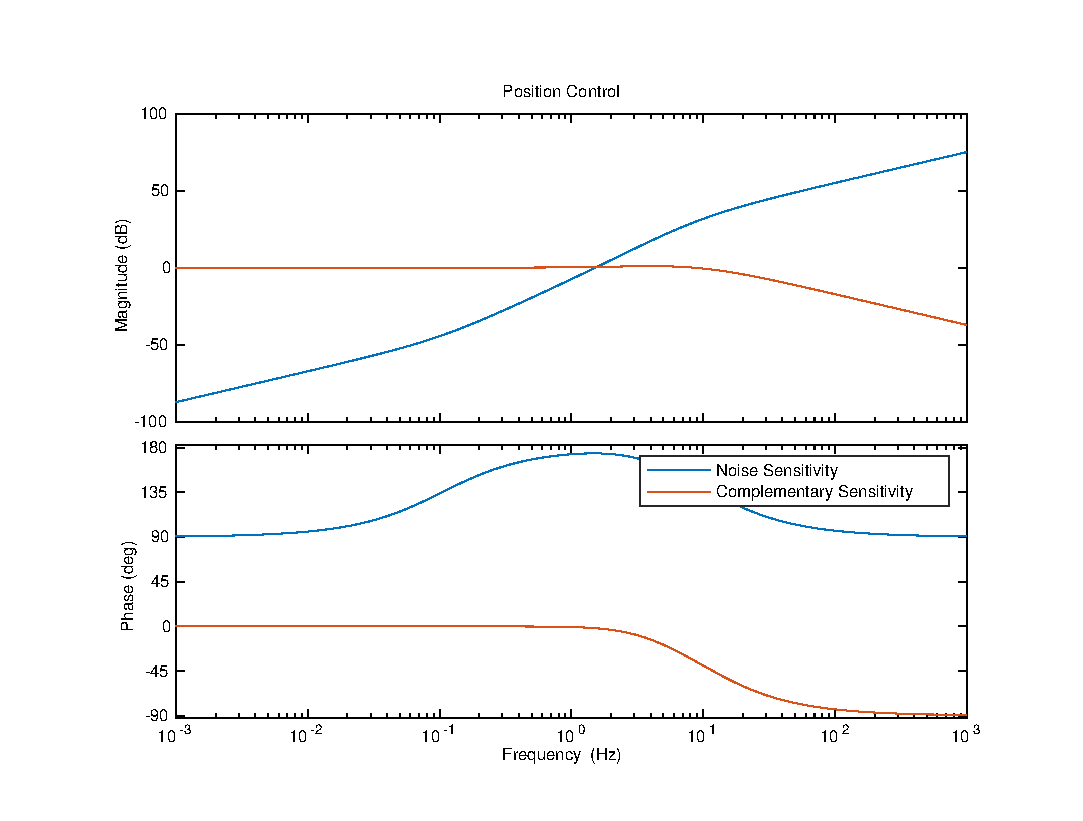
\includegraphics[width=0.8\textwidth]{images/position_tf.eps}
\end{center}
\caption{Position control bode plot of the complementary sensitivity function and noise sensitivity function}
\label{fig:position_tf}
\end{figure}

\newpage

\subsubsection{Modulated reference}
\noindent As it is visible the reference requires high current in order to be performed, the code scaled the signal as soon as we reached the saturation in order to guarantee the saturation limits.

\begin{figure}[H]
\begin{center}
\hspace*{-5cm}
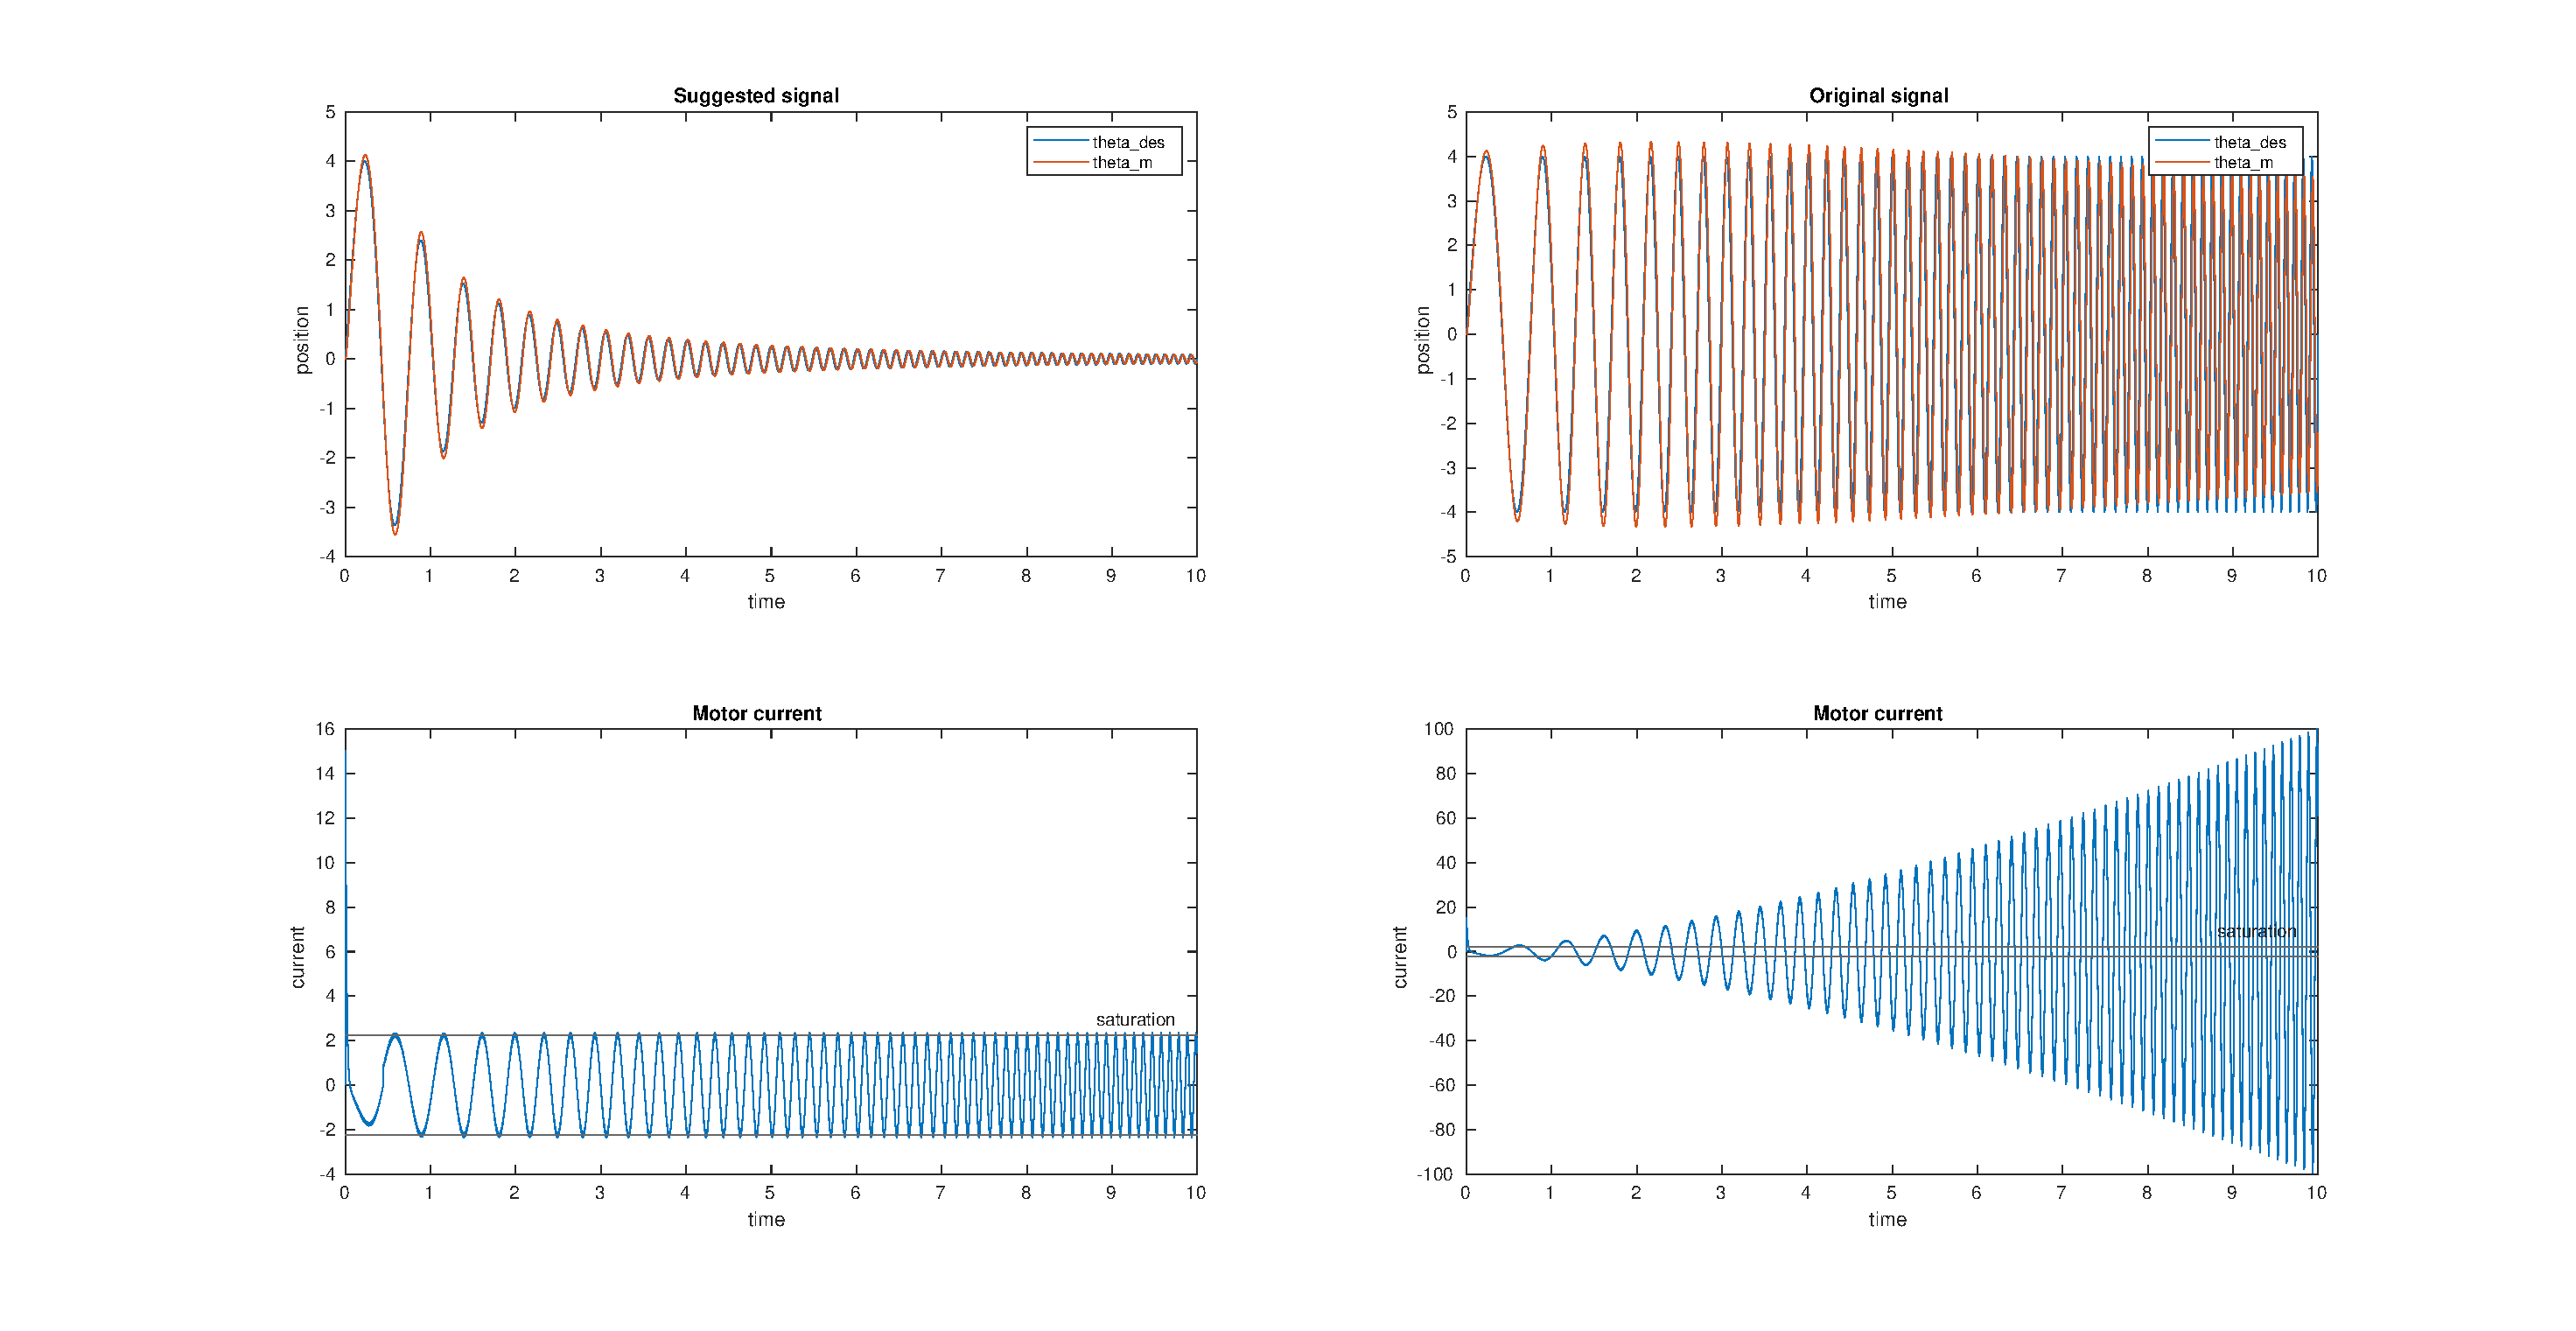
\includegraphics[width=1.6\textwidth]{images/position_tau2.eps}
\end{center}
\caption{Comparison of the original position signal with the suggested saturation aware one}
\label{fig:position_tau}
\end{figure}

To obtain Fig \ref{fig:position_tau} a PD with $P = 10$ and $D = 0.9$ was used. The current saturation is $2.26$A, and the sweep signal goes from 1 to 10 Hz in 10 seconds. The motor used is the one described in the parameters section.

\newpage
\subsection{Velocity Control}
Let's consider a basic velocity control architecture for a linear motor model considering only the mechanical subsystem. The related equations of the plant $P_l$ and the PI controller $C$ are:

\[
P_l = \frac{1}{J_m s + d_m} \qquad
C = P + \frac{I}{s}
\]

\bigskip
\noindent The two transfer functions $T(S)$ ($r$ to $y$) and $CS(s)$ ($r$ to $u$) are presented in Fig \ref{fig:velocity_tf}.

\begin{figure}[H]
  \begin{center}
  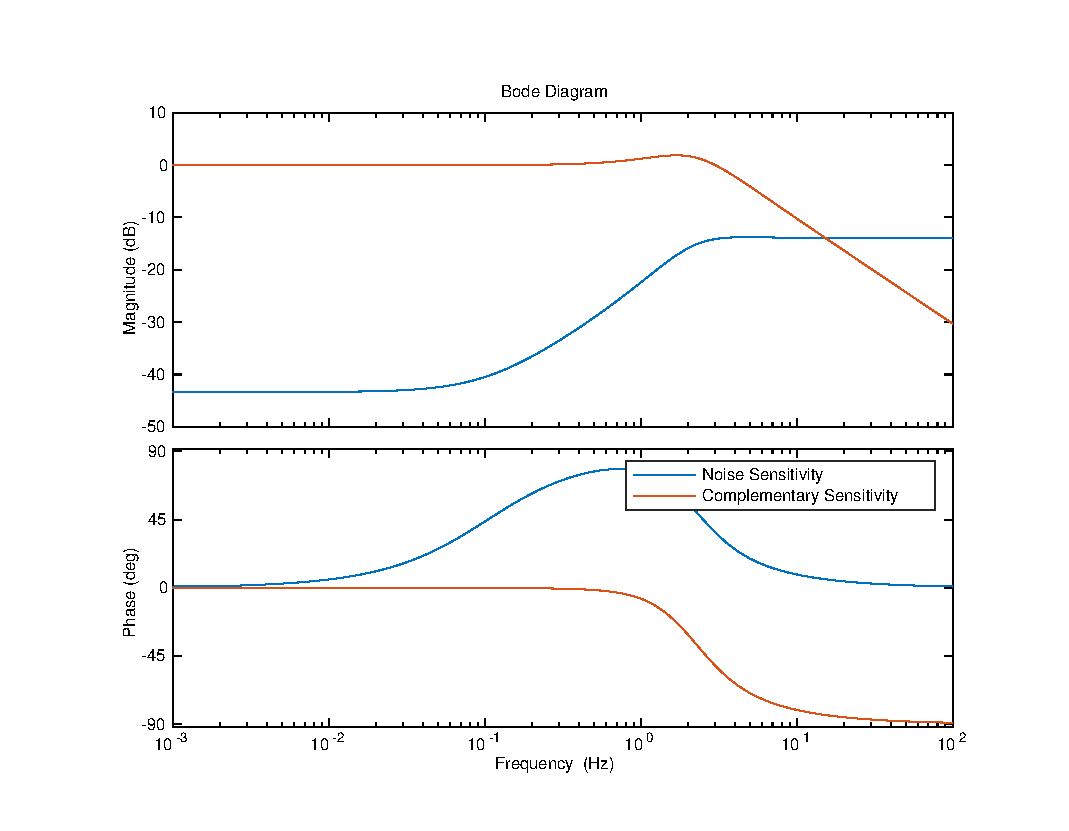
\includegraphics[width=0.8\textwidth]{images/velocity_tf.eps}
  \end{center}
  \caption{Velocity control bode plot of the complementary sensitivity function and noise sensitivity function}
  \label{fig:velocity_tf}
  \end{figure}
\bigskip 

It is important to notice that the noise sensitivity function in Fig \ref{fig:velocity_tf} doesn't reach the 0db level so it means we can't reach saturation with unitary references. However the amplitude of the reference (when > 1) will shift the transfer function and it will eventually reach 0db leading to current saturation.

\newpage
\subsubsection{Modulated reference}
\noindent As it is visible the reference requires high current in order to be performed, the code scaled the signal as soon as we reached the saturation in order to guarantee the saturation limits.
\begin{figure}[H]
  \begin{center}
  \hspace*{-5cm}
  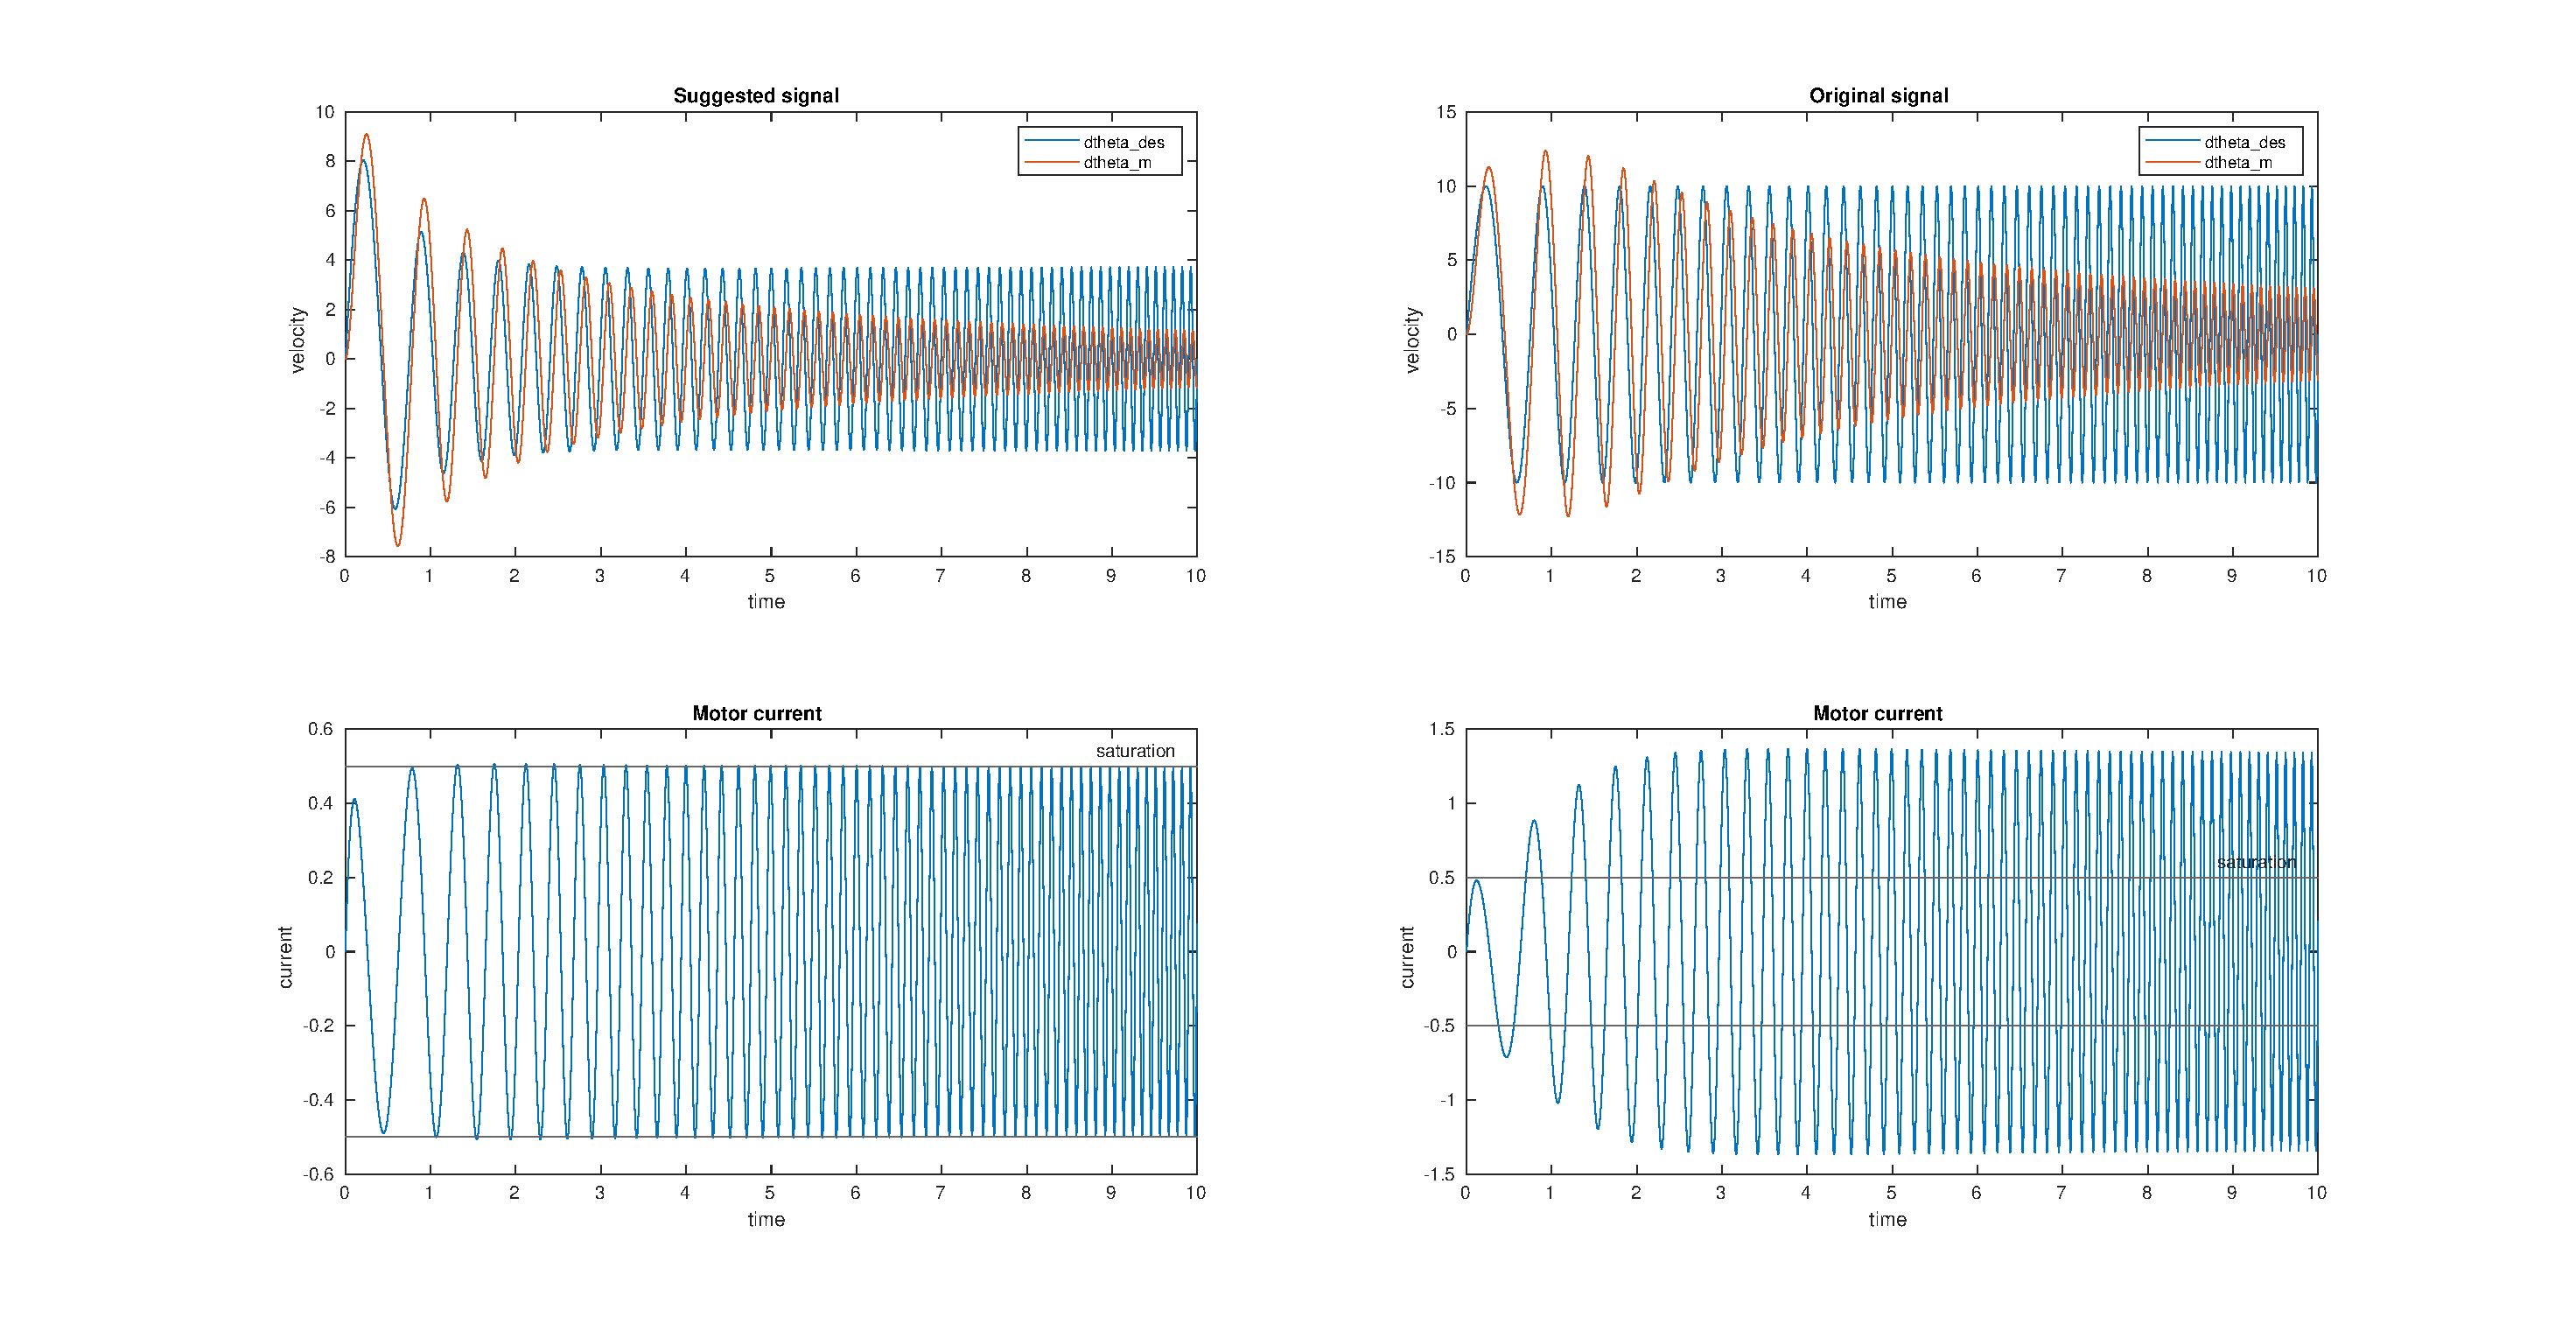
\includegraphics[width=1.6\textwidth]{images/velocity_tau.eps}
  \end{center}
  \caption{Comparison of the original velocity signal with the suggested saturation aware one}
  \label{fig:velocity_tau}
  \end{figure}

  To obtain Fig \ref{fig:velocity_tau} a PD with $P = 0.2$ and $I = 2$ was used. The current saturation is $0.5$A, and the sweep signal goes from 1 to 10 Hz in 10 seconds. The motor used is the one described in the parameters section.

\newpage
\subsection{Basic Force Control}
Let's consider a basic force control architecture for a linear motor model considering only the mechanical subsystem and a PD controller. I will assume only some stiffness $h$ following the analysis in \cite{eppinger}. The related equations of the plant $P_l$ and the PD controller $C$ are:

\[
G = P_{l} = \frac{1}{\frac{J_m}{h}s^2 + \frac{d_m}{h}s + 1} \qquad
C = P + Ds;                             
\]

\bigskip
\begin{figure}[H]
\begin{center}
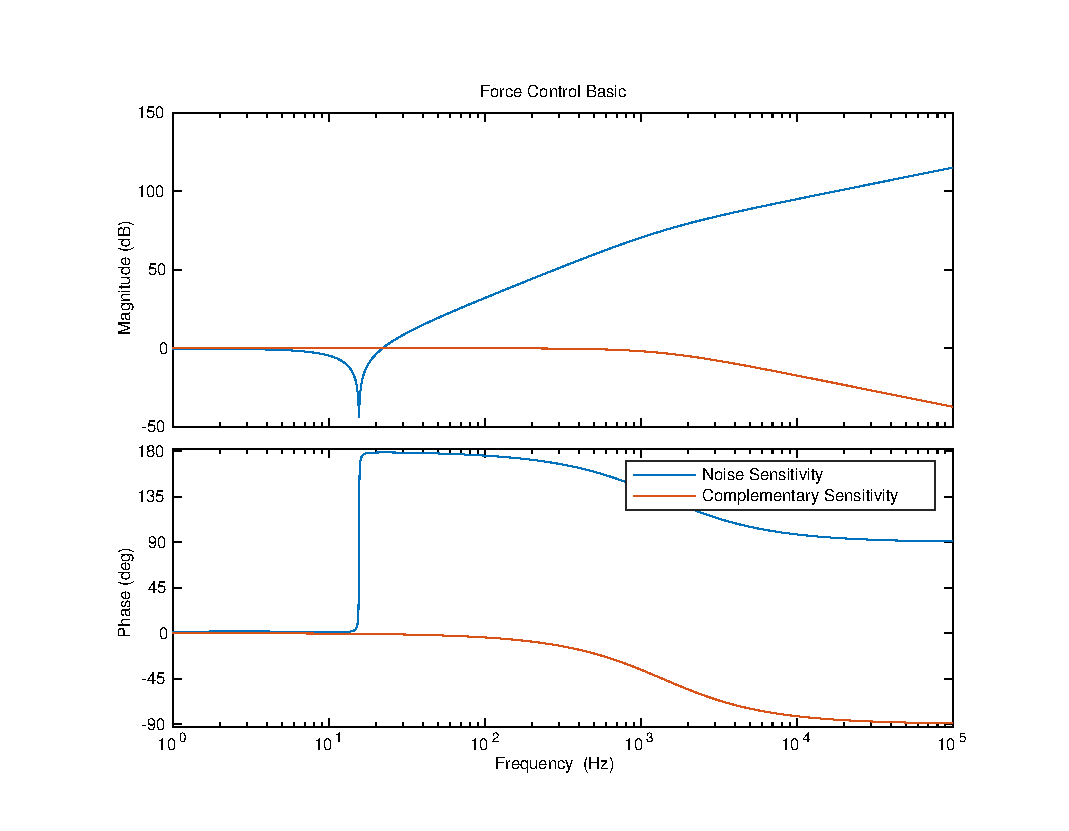
\includegraphics[width=0.8\textwidth]{images/force_tf.eps}
\end{center}
\caption{Force control bode plot of the complementary sensitivity function and noise sensitivity function}
\label{fig:force_tf}
\end{figure}

\bigskip 
It is important to notice that the peak in the noise sensitivity function in Fig \ref{fig:force_tf} depends on the stiffness of the environment and it can't be eliminated. However our method consider the amplification only when the transfer function exceeds 0db so the peak is always neglected.

\newpage
\subsubsection{Modulated reference}
\noindent As it is visible the reference requires high current in order to be performed, the code scaled the signal as soon as we reached the saturation in order to guarantee the saturation limits.
\begin{figure}[H]
  \begin{center}
  \hspace*{-5cm}
  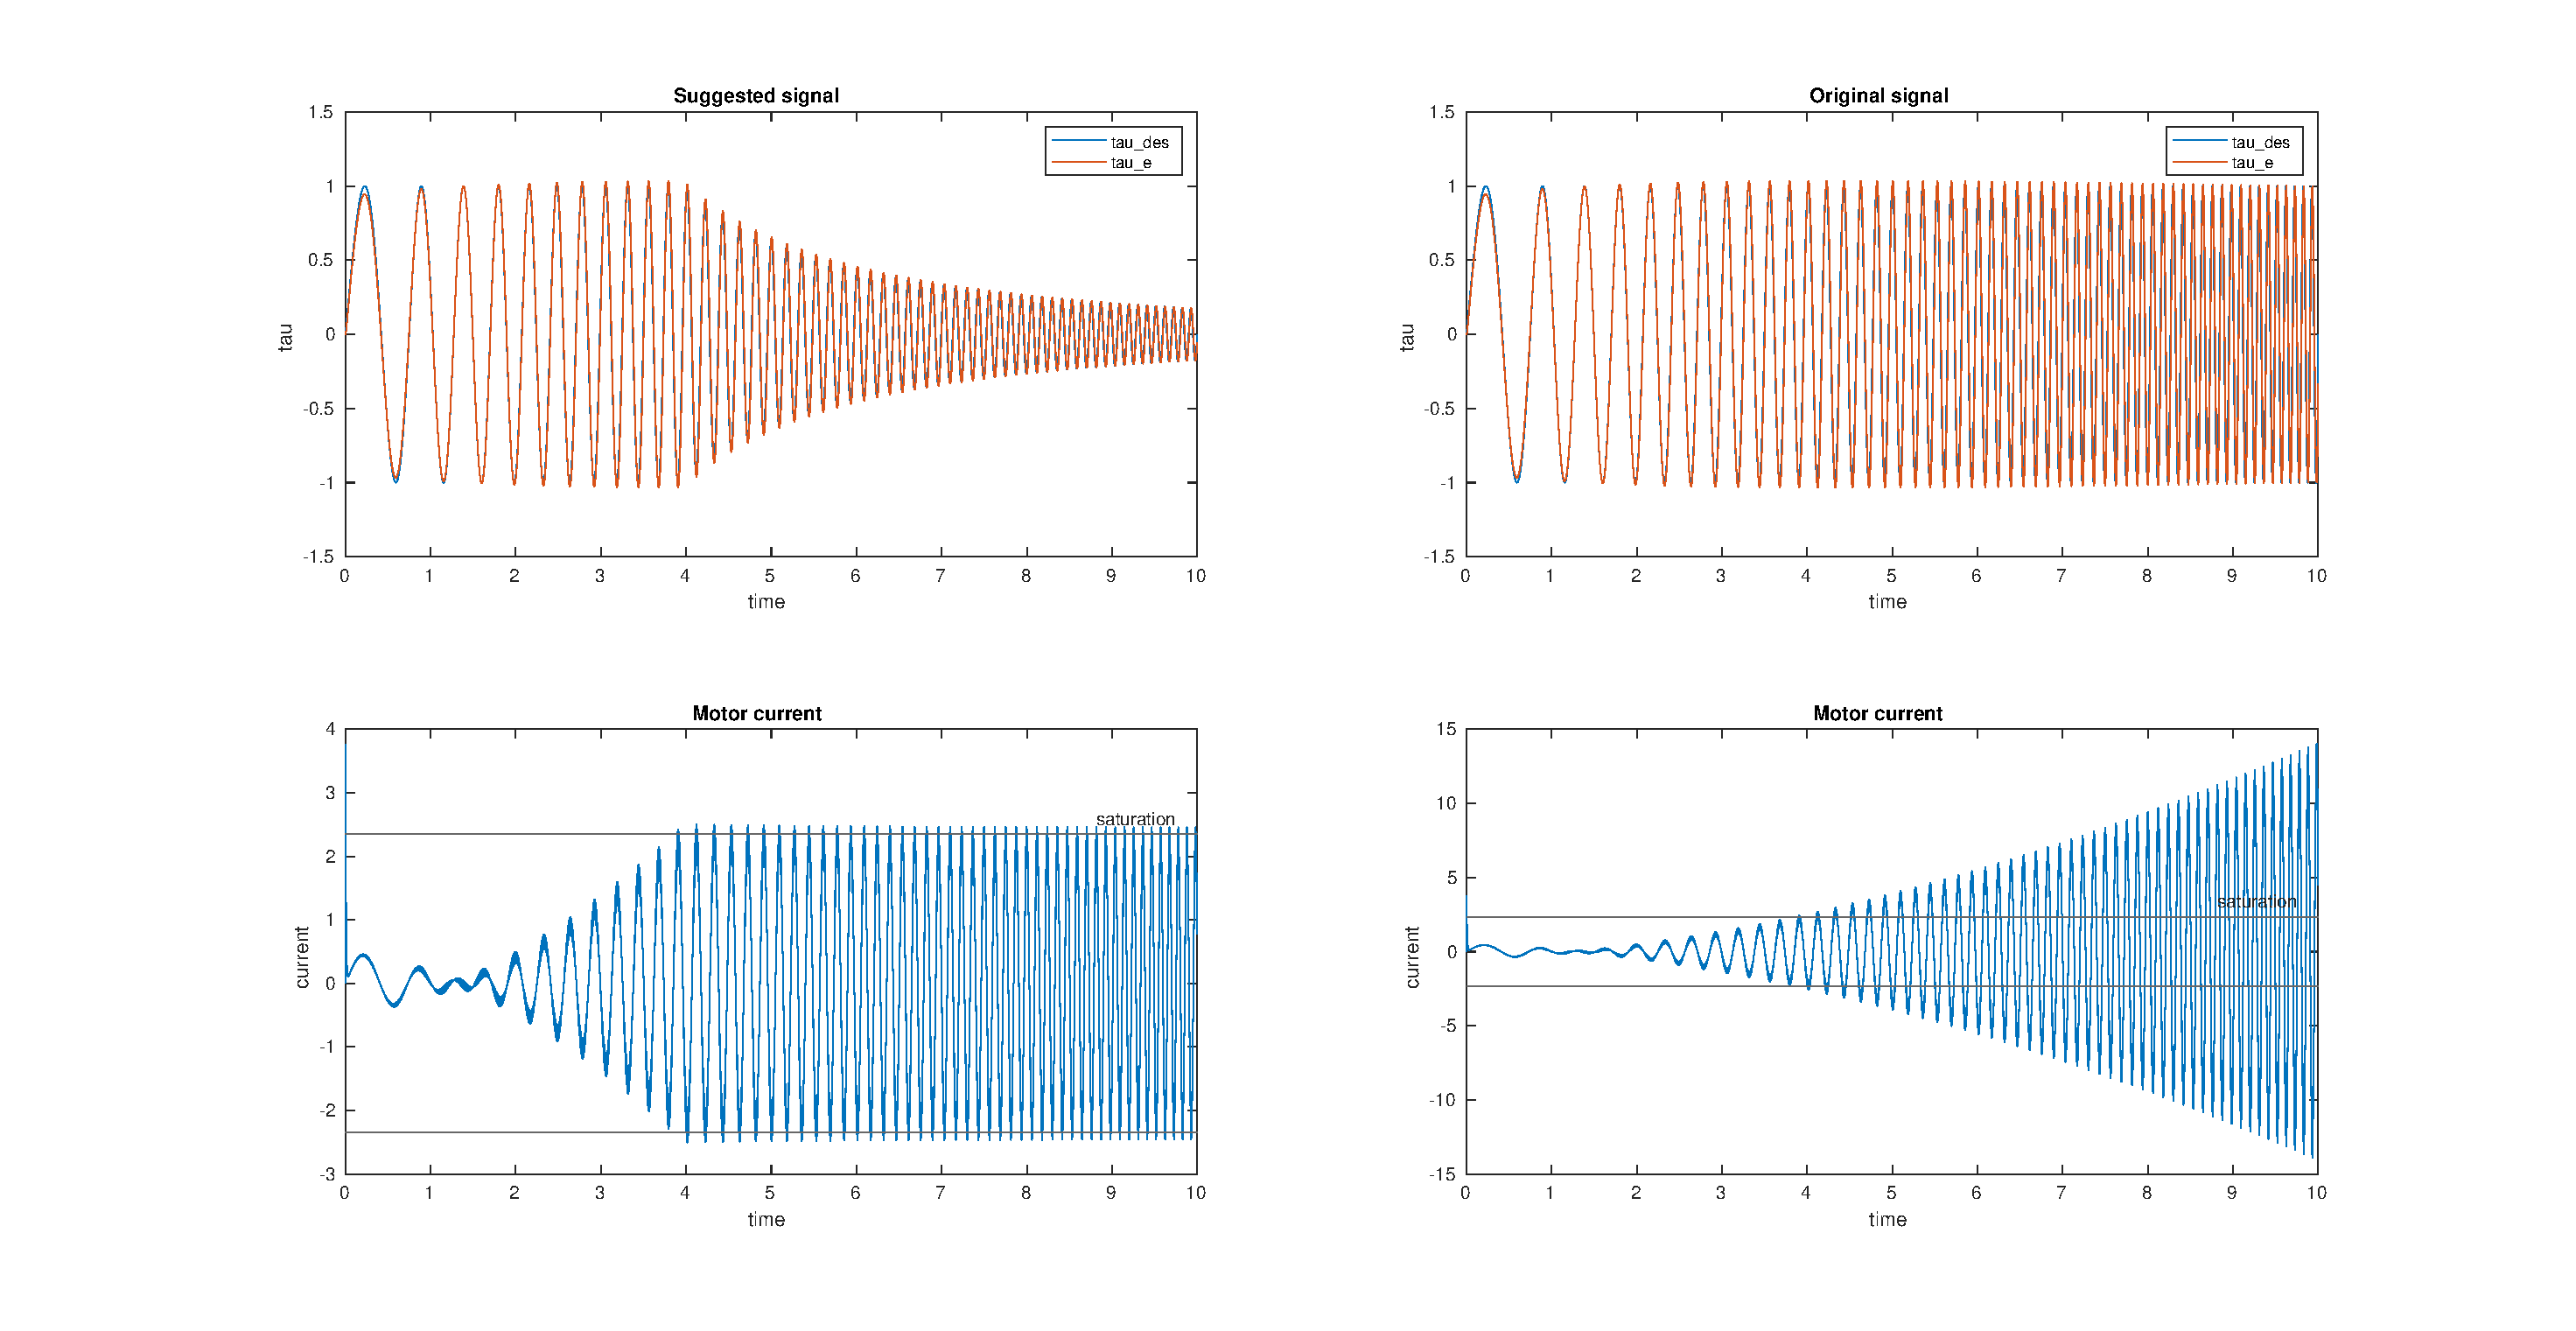
\includegraphics[width=1.6\textwidth]{images/force_tau.eps}
  \end{center}
  \caption{Comparison of the original force signal with the suggested saturation aware one}
  \label{fig:force_tau}
  \end{figure}

  To obtain Fig \ref{fig:force_tau} a PD with $P = 10$ and $D = 0.9$ was used. The current saturation is $2.26$A, and the sweep signal goes from 1 to 10 Hz in 10 seconds. The motor used is the one described in the parameters section. The stiffness of the environment is $2Nm/rad$.

\section{Limitations}

The current approach based on the use of the transfer function $CS(s)$ has lots of limitations:
\begin{itemize}
  \item The approach assumes full knowledge of the considered system, everything has to be identified correctly and this is even a bigger limitation for force control because we don't have informations about the environment which makes the use of the transfer functions not reliable at all.
  \item We assume a linear system which is a big limitation since it doesn't consider non-linear behaviours of the DC motors. For this cases having at least one real experiment to validate the data is a must.
\end{itemize}

\section{Other approaches}

Simulating the experiments in simulink is in general a good way to verify the presence of saturation but it is affected by the same problems related to prior knowledge and linear behaviours (at least without implementing a non-linear system). A good way to generate a current saturation aware reference signal is adapting the reference in real time by reading directly the current provided to the motor. If this exceeds a certain threasold just drop a certain percentage. The bandwith estimation can be performed using the Matlab toolbox over that data.

\section{Conclusions}
The report is an attempt to provide a way to generate current saturation aware signals using noise sensitivity trasfer function. The reported approach is pretty flexible and can be extended to guarantee also voltage or velocity limits as in \cite{Performance}. The basic idea was provided as well as some simulation results. The main limitations and other possibilities were discussed and analysed.

\begin{thebibliography}{9}

\bibitem{Forecast}
Forecast Project https://eurobench2020.eu/developing-the-framework/force-control-algorithms-testbench-forecast/

\bibitem{scientist}
Karl Johan Astrom, Richard M. Murray Feedback Systems An Introduction for Scientists and Engineers

\bibitem{Performance}
Chan Lee, Sehoon Oh Performance Analysis of Series Elastic Actuator based on Maximum Torque Transmissibility

\bibitem{eppinger}
Eppinger, Seering Introduction to Dynamic Models for Robot Force Control 
\end{thebibliography}
\end{document}


